\documentclass{article}
\usepackage{tikz}
\usetikzlibrary{automata,positioning}

\begin{document}

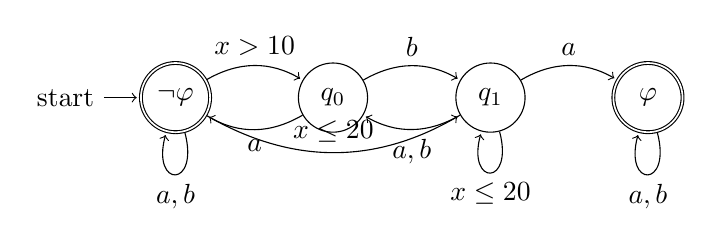
\begin{tikzpicture}[shorten >=1pt,node distance=2cm,on grid,auto]
    \node[state,initial,accepting] (q_0) {$\neg\varphi$};
    \node[state] (q_1) [right=of q_0] {$q_0$};
    \node[state] (q_2) [right=of q_1] {$q_1$};
    \node[state,accepting] (q_3) [right=of q_2] {$\varphi$};

    \path[->]
        (q_0) edge [loop below] node {$a,b$} ()
              edge [bend left] node {$x>10$} (q_1)
              edge [bend right] node {$x\leq 20$} (q_2)
        (q_1) edge [bend left] node {$a$} (q_0)
              edge [bend left] node {$b$} (q_2)
        (q_2) edge [loop below] node {$x\leq 20$} ()
              edge [bend left] node {$a$} (q_3)
              edge [bend left] node {$a,b$} (q_1)
        (q_3) edge [loop below] node {$a,b$} ();
\end{tikzpicture}

\end{document}